\documentclass[tikz,border=6pt]{standalone}
\usepackage[utf8]{inputenc}
\usepackage[T1]{fontenc}
\usepackage{amsmath,amssymb,bm}
\usepackage{lmodern}
\usetikzlibrary{arrows.meta,positioning,calc}

\definecolor{ink}{HTML}{1d1d1f}
\definecolor{graytext}{HTML}{515154}
\definecolor{muted}{HTML}{86868b}
\definecolor{linegray}{HTML}{d2d2d7}
\definecolor{blueaccent}{HTML}{2997ff}
\definecolor{amber}{HTML}{ff9f0a}
\definecolor{amberdark}{HTML}{c76008}
\definecolor{greenaccent}{HTML}{30d158}
\definecolor{greendark}{HTML}{1a7f37}
\definecolor{redaccent}{HTML}{ff453a}
\definecolor{reddark}{HTML}{d70015}

\begin{document}
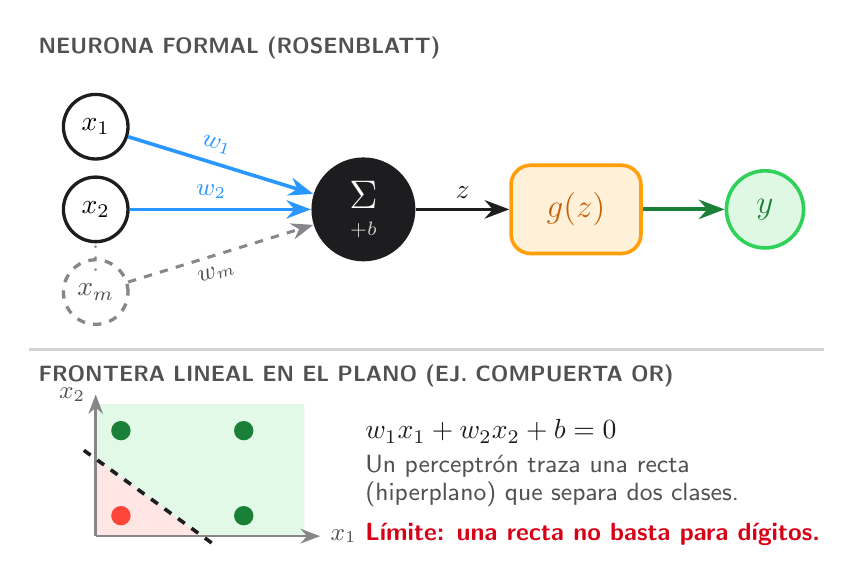
\begin{tikzpicture}[
  font=\sffamily,
  >=Stealth,
  innode/.style={circle,draw=ink,fill=white,line width=1.2pt,minimum size=0.82cm,inner sep=0pt,font=\sffamily\bfseries\normalsize},
  sum/.style={circle,fill=ink,text=white,minimum size=1.32cm,inner sep=0pt,align=center},
  act/.style={rectangle,rounded corners=7pt,draw=amber,fill=amber!16,line width=1.3pt,minimum width=1.65cm,minimum height=1.12cm,text=amberdark,font=\sffamily\bfseries\large},
  outnode/.style={circle,draw=greenaccent,fill=greenaccent!16,line width=1.3pt,minimum size=0.98cm,text=greendark,font=\sffamily\bfseries\large}
]

% Sección superior: Neurona formal
\node[anchor=west,font=\sffamily\bfseries\footnotesize,text=graytext] at (0,5.25) {NEURONA FORMAL (ROSENBLATT)};

\node[innode] (x1) at (0.85,4.25) {$x_1$};
\node[innode] (x2) at (0.85,3.20) {$x_2$};
\node[innode,draw=muted,dashed,text=graytext] (xm) at (0.85,2.15) {$x_m$};
\node[font=\small,text=muted] at (0.85,2.68) {$\vdots$};

\node[sum] (sum) at (4.25,3.20) {\Large$\Sigma$\\[-2pt]\scriptsize\color{gray!40}$+b$};
\node[act] (g) at (6.95,3.20) {$g(z)$};
\node[outnode] (y) at (9.35,3.20) {$y$};

\draw[->,blueaccent,line width=1.3pt] (x1) -- node[above,sloped,pos=0.45,font=\small\bfseries,text=blueaccent]{$w_1$} (sum);
\draw[->,blueaccent,line width=1.3pt] (x2) -- node[above,pos=0.45,font=\small\bfseries,text=blueaccent]{$w_2$} (sum);
\draw[->,muted,dashed,line width=1.1pt] (xm) -- node[below,sloped,pos=0.45,font=\small\bfseries,text=graytext]{$w_m$} (sum);

\draw[->,ink,line width=1.3pt] (sum) -- node[above,font=\normalsize]{$z$} (g);
\draw[->,greendark,line width=1.4pt] (g) -- (y);

% Divisor horizontal
\draw[linegray,line width=0.8pt] (0,1.42) -- (10.1,1.42);

% Sección inferior: Compuerta OR
\node[anchor=west,font=\sffamily\bfseries\footnotesize,text=graytext] at (0,1.08) {FRONTERA LINEAL EN EL PLANO (EJ.\ COMPUERTA OR)};

\begin{scope}[shift={(0.45,-1.15)}]
  \fill[redaccent!14] (0.4,0.2) -- (0.4,1.18) -- (1.75,0.2) -- cycle;
  \fill[greenaccent!14] (0.4,1.18) -- (0.4,1.88) -- (3.05,1.88) -- (3.05,0.2) -- (1.75,0.2) -- cycle;
  \draw[->,muted,line width=0.9pt] (0.4,0.2) -- (3.25,0.2) node[right,font=\small,text=graytext]{$x_1$};
  \draw[->,muted,line width=0.9pt] (0.4,0.2) -- (0.4,2.0) node[left,font=\small,text=graytext]{$x_2$};
  \draw[ink,line width=1.3pt,dashed] (0.25,1.29) -- (1.92,0.08);
  \fill[redaccent] (0.72,0.46) circle (3.5pt);
  \fill[greendark] (0.72,1.54) circle (3.5pt);
  \fill[greendark] (2.28,0.46) circle (3.5pt);
  \fill[greendark] (2.28,1.54) circle (3.5pt);
\end{scope}

\node[anchor=west,font=\sffamily\bfseries\normalsize,text=ink] at (4.15,0.38) {$w_1 x_1 + w_2 x_2 + b = 0$};
\node[anchor=west,font=\sffamily\small,text=graytext,align=left] at (4.15,-0.25) {Un perceptrón traza una recta\\[-1pt](hiperplano) que separa dos clases.};
\node[anchor=west,font=\sffamily\bfseries\small,text=reddark] at (4.15,-0.92) {Límite: una recta no basta para dígitos.};

\end{tikzpicture}
\end{document}
